\documentclass[]{llncs} 
\usepackage{amsmath}
\usepackage{verbatim}
\usepackage{datatool}
\usepackage{tikz}
\usetikzlibrary{arrows,shapes}
\usepackage{graphics}

%\newtheorem{theorem}{Theorem}

\newcommand{\TODO}[1]{ {\color{red}{#1} }}
\newcommand{\com}[1]{ {\color{blue}{--- #1 ---}}}

\author{Valentin Mayer-Eichberger}

\institute{NICTA \\ University of New South Wales \\
\email{valentin.mayer-eichberger@nicta.com.au}}

\title{A SAT Encoding for the AtMostSeqCard Constraint}

\begin{document} \maketitle

\section{Introduction}

Give description of the car sequencing problem and the straight
forward encoding in IP/CNF. 

The naive CNF and IP encoding of the car sequencing benchmark is
far from optimal. In this paper we will show gradually how to come up
with a better encoding. 

\section{Motivation}

We are seeking an encoding that enforces GAC on the recently proposed
AtMostSeqCard constraint (\TODO{ref}). This constraint is not as expressive as the
Sequence constraint but is more suited for some benchmark problems and
has a linear filtering algorithm. Here we will show that there is a
compact CNF encoding that shows good results in the benchmark set of the
CSPLIB. Furthermore we will try to improve the bounds on the set of hard
instance. 

\section{Encoding of one AtMostSeqCard}

We will first show how to encode a cardinality constraint with a counter
encoding (\TODO{ref}) and then integrate the AtMostSeq by reusing the auxiliary
variables of the counter encoding. 

Over this whole section we will work with the following notation. Given
a set of consecutive positions $P=\{1\ldots n\}$ and a property (class
or option) $i$. Let $x_{i,j}$ be true iff property $i$ is true at
position $j$. In this section we embedd one counter for one property
$i$, so $i$ is fixed over the whole section. The interaction with other
properties is shown in the subsequent section. 

\subsection{Encoding of Counters}

We want to encode the following cardinality constraint

$$ \sum_{j\in P} x_{i,j} = d $$

where $d$ is a fixed value.  We call the encoding for such a cardinality
constraint a counter encoding because we count exactly $d$ occurences of
property $i$ over positions $P$. 

So given an option or a class identified by subscript $i\in I$ that
needs to be counted over sequence of positions $P$. We introduce the
following variables: 

\begin{itemize}
    \item $y_{i,j,k}$ is true iff at least $k$ times holds property $i$
        in the positions $0 \ldots j $. 
\end{itemize}

Notice that we assume the set $P$ to have a total ordering. We count
along this ordering. The following formula clearifies the relationship
between $x$ and $y$.

$$ y_{i,j,k} \iff (k \leq \sum_{l=0}^{j} x_{i,l}) $$


\begin{figure}
\centering 
\caption{The variables $y_{i,j,k}$ for a countable property $i$ with an
upper bound of two over a sequence of 10. The variables corresponding to
the cells containing $U$($L$) are set to false (true). The question mark
identifies a unassigned variable of the counter encoding}
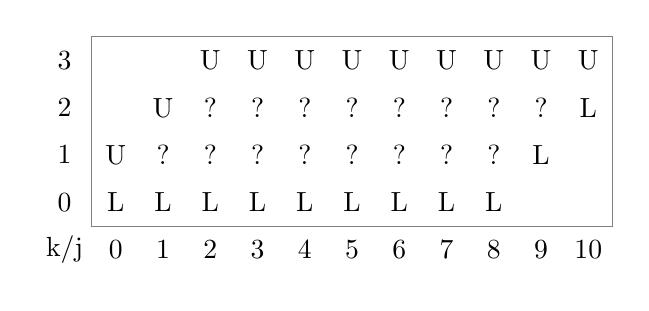
\begin{tikzpicture}
\node [matrix,ampersand replacement=\&,nodes={minimum size=6mm}]
%,nodes={fill=blue!20,minimum size=5mm}] 
    {
        \node {3}; \& \node (x) { }; \& \node { }; \& \node {U}; \& \node {U}; \& \node {U}; \& \node {U}; \& \node {U}; \& \node {U}; \& \node {U}; \& \node {U}; \& \node {U}; \\
        \node {2}; \& \node { }; \& \node {U}; \& \node {?}; \& \node {?}; \& \node {?}; \& \node {?}; \& \node {?}; \& \node {?}; \& \node {?}; \& \node {?}; \& \node {L}; \\
        \node {1}; \& \node {U}; \& \node {?}; \& \node {?}; \& \node {?}; \& \node {?}; \& \node {?}; \& \node {?}; \& \node {?}; \& \node {?}; \& \node {L}; \& \node { }; \\
        \node {0}; \& \node {L}; \& \node {L}; \& \node {L}; \& \node {L}; \& \node {L}; \& \node {L}; \& \node {L}; \& \node {L}; \& \node {L}; \& \node { }; \& \node (y) { }; \\
        \node {k/j}; \& \node {0}; \& \node {1}; \& \node {2}; \& \node {3}; \& \node {4}; \& \node {5}; \& \node {6}; \& \node {7}; \& \node {8}; \& \node {9}; \& \node {10}; \\
};
\draw[gray] (x.north west) rectangle (y.south east);
\end{tikzpicture}
\end{figure}

There are two types of binay clauses that relate the variables $y$ among
each other and two types of tenery clauses that coordinate $y$ with the
variables $x$.

\begin{equation}
    \bigwedge_{\substack{j \in P \\ j+1\in P}} \bigwedge_{k\in\{1..d\}}
    \neg y_{i,j,k} \vee y_{i,j+1,k}
\end{equation}

\begin{equation}
    \bigwedge_{\substack{j \in P \\ j-1\in P}} \bigwedge_{k,k-1\in\{1..d\}}
    \neg y_{i,j,k} \vee y_{i,j-1,k-1}
\end{equation}

These clauses restrict the structure of the auxiliary variables to
consist of a counter. Now we need to relate these variables to $x$. 
First we define clauses that consist of pushing the counter up. 

\begin{equation}
    \bigwedge_{\substack{j \in P \\ j+1\in P}} \bigwedge_{k,k+1\in\{0..d+1\}}
    \neg x_{i,j} \vee \neg y_{i,j,k} \vee y_{i,j+1,k+1}
\end{equation}

And now we have to restrict the counter to be pushed up if $x_{i,j}$ is
false. 

\begin{equation}
    \bigwedge_{\substack{j \in P \\ j+1\in P}} \bigwedge_{k,k+1\in\{1..d+1\}}
    \neg x_{i,j} \vee \neg y_{i,j,k} \vee y_{i,j+1,k+1}
\end{equation}



\begin{figure}
\centering 
\caption{Taking the previous example and let $x_{i,j}$ be true for
    position 2 and 7. Then the resulting assignment to the counter
    variable is given in this table. }
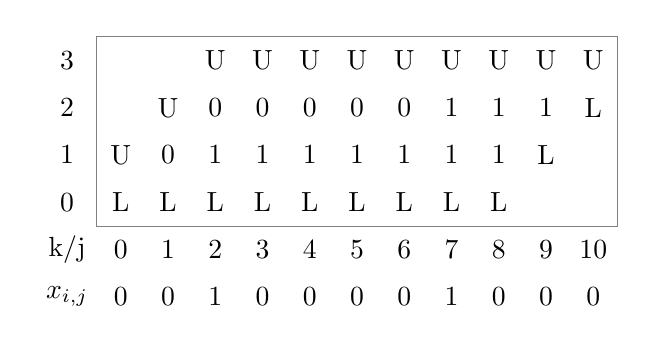
\begin{tikzpicture}
\node [matrix,ampersand replacement=\&,nodes={minimum size=6mm}]
%,nodes={fill=blue!20,minimum size=5mm}] 
    {
        \node {3}; \& \node (x) { }; \& \node { }; \& \node {U}; \& \node {U}; \& \node {U}; \& \node {U}; \& \node {U}; \& \node {U}; \& \node {U}; \& \node {U}; \& \node {U}; \\
        \node {2}; \& \node { }; \& \node {U}; \& \node {0}; \& \node {0}; \& \node {0}; \& \node {0}; \& \node {0}; \& \node {1}; \& \node {1}; \& \node {1}; \& \node {L}; \\
        \node {1}; \& \node {U}; \& \node {0}; \& \node {1}; \& \node {1}; \& \node {1}; \& \node {1}; \& \node {1}; \& \node {1}; \& \node {1}; \& \node {L}; \& \node { }; \\
        \node {0}; \& \node {L}; \& \node {L}; \& \node {L}; \& \node {L}; \& \node {L}; \& \node {L}; \& \node {L}; \& \node {L}; \& \node {L}; \& \node { }; \& \node (y) { }; \\
        \node {k/j}; \& \node {0}; \& \node {1}; \& \node {2}; \& \node {3}; \& \node {4}; \& \node {5}; \& \node {6}; \& \node {7}; \& \node {8}; \& \node {9}; \& \node {10}; \\
        \node {$x_{i,j}$}; \& \node {0}; \& \node {0}; \& \node {1}; \& \node {0}; \& \node {0}; \& \node {0}; \& \node {0}; \& \node {1}; \& \node {0}; \& \node {0}; \& \node {0}; \\
};
\draw[gray] (x.north west) rectangle (y.south east);
\end{tikzpicture}
\end{figure}

\subsection{Extending to AtMostSeqCard}

Given a sequence of boolean variables among exactly $d$ have to be true
and each window of size $q$ cannot contain more than $u$ true variables.
This is the AtMostSeqCard constraint: 

$$ \text{AtMostSeqCard}(u,q,d,[x_{i,1},\ldots,x_{i,n}]) \iff
\bigwedge_{j=0}^{n-q}(\sum_{l=1}^q x_{i,j+l} \leq u ) \wedge (\sum_{j=1}^n
x_{i,j} = d) $$

To archive GAC on this constraint we need to take the counter encoding
of the previous section and add the following binary clauses:

\begin{equation}
    \bigwedge_{\substack{j \in P \\ j-q\in P}}
    \bigwedge_{\substack{k\in\{1..d\}\\ k-u \in \{1..d\}}}
    \neg y_{i,j,k} \vee y_{i,j-q,k-u}
\end{equation}

\begin{theorem}
The clauses of (1) to (5) enforce GAC on the AtMostSeqCard for all
partial assignment on variables $x_{i,j,}$. 
\end{theorem}

The power of the binary clauses are best shown in the example taken from
(\TODO{ref})

\begin{figure}
\centering 
\caption{Taking the inital state of the propagator for a constraint with
$u=4,q=8,d=12,n=22$. In this example we see that already $x_{i,7}$,
$x_{i,8}$, $x_{i,15}$ and $x_{i,16}$ need to be set to false. Notice
that for this particular case we only need 24 boolean variables to
create the GAC encoding.}
\begin{tikzpicture}
\node [matrix,ampersand replacement=\&,nodes={minimum size=6mm}]
%,nodes={fill=blue!20,minimum size=5mm}] 
    {
\node{13}; \& \node (x) { }; \& \node { }; \& \node { }; \& \node { }; \& \node { }; \& \node { }; \& \node { }; \& \node { }; \& \node { }; \& \node { }; \& \node { }; \& \node { }; \& \node { }; \& \node { }; \& \node { }; \& \node { }; \& \node { }; \& \node { }; \& \node { }; \& \node { }; \& \node {U}; \& \node {U}; \& \node {U}; \\
\node{12}; \& \node { }; \& \node { }; \& \node { }; \& \node { }; \& \node { }; \& \node { }; \& \node { }; \& \node { }; \& \node { }; \& \node { }; \& \node { }; \& \node { }; \& \node { }; \& \node { }; \& \node { }; \& \node { }; \& \node { }; \& \node { }; \& \node { }; \& \node {U}; \& \node {?}; \& \node {?}; \& \node {L}; \\
\node{11}; \& \node { }; \& \node { }; \& \node { }; \& \node { }; \& \node { }; \& \node { }; \& \node { }; \& \node { }; \& \node { }; \& \node { }; \& \node { }; \& \node { }; \& \node { }; \& \node { }; \& \node { }; \& \node { }; \& \node { }; \& \node { }; \& \node {U}; \& \node {?}; \& \node {?}; \& \node {L}; \& \node { }; \\
\node{10}; \& \node { }; \& \node { }; \& \node { }; \& \node { }; \& \node { }; \& \node { }; \& \node { }; \& \node { }; \& \node { }; \& \node { }; \& \node { }; \& \node { }; \& \node { }; \& \node { }; \& \node { }; \& \node { }; \& \node { }; \& \node {U}; \& \node {?}; \& \node {?}; \& \node {L}; \& \node { }; \& \node { }; \\
\node{9}; \& \node { }; \& \node { }; \& \node { }; \& \node { }; \& \node { }; \& \node { }; \& \node { }; \& \node { }; \& \node { }; \& \node { }; \& \node { }; \& \node { }; \& \node {U}; \& \node {U}; \& \node {U}; \& \node {U}; \& \node {U}; \& \node {?}; \& \node {?}; \& \node {L}; \& \node { }; \& \node { }; \& \node { }; \\
\node{8}; \& \node { }; \& \node { }; \& \node { }; \& \node { }; \& \node { }; \& \node { }; \& \node { }; \& \node { }; \& \node { }; \& \node { }; \& \node { }; \& \node {U}; \& \node {?}; \& \node {?}; \& \node {L}; \& \node {L}; \& \node {L}; \& \node {L}; \& \node {L}; \& \node { }; \& \node { }; \& \node { }; \& \node { }; \\
\node{7}; \& \node { }; \& \node { }; \& \node { }; \& \node { }; \& \node { }; \& \node { }; \& \node { }; \& \node { }; \& \node { }; \& \node { }; \& \node {U}; \& \node {?}; \& \node {?}; \& \node {L}; \& \node { }; \& \node { }; \& \node { }; \& \node { }; \& \node { }; \& \node { }; \& \node { }; \& \node { }; \& \node { }; \\
\node{6}; \& \node { }; \& \node { }; \& \node { }; \& \node { }; \& \node { }; \& \node { }; \& \node { }; \& \node { }; \& \node { }; \& \node {U}; \& \node {?}; \& \node {?}; \& \node {L}; \& \node { }; \& \node { }; \& \node { }; \& \node { }; \& \node { }; \& \node { }; \& \node { }; \& \node { }; \& \node { }; \& \node { }; \\
\node{5}; \& \node { }; \& \node { }; \& \node { }; \& \node { }; \& \node {U}; \& \node {U}; \& \node {U}; \& \node {U}; \& \node {U}; \& \node {?}; \& \node {?}; \& \node {L}; \& \node { }; \& \node { }; \& \node { }; \& \node { }; \& \node { }; \& \node { }; \& \node { }; \& \node { }; \& \node { }; \& \node { }; \& \node { }; \\
\node{4}; \& \node { }; \& \node { }; \& \node { }; \& \node {U}; \& \node {?}; \& \node {?}; \& \node {L}; \& \node {L}; \& \node {L}; \& \node {L}; \& \node {L}; \& \node { }; \& \node { }; \& \node { }; \& \node { }; \& \node { }; \& \node { }; \& \node { }; \& \node { }; \& \node { }; \& \node { }; \& \node { }; \& \node { }; \\
\node{3}; \& \node { }; \& \node { }; \& \node {U}; \& \node {?}; \& \node {?}; \& \node {L}; \& \node { }; \& \node { }; \& \node { }; \& \node { }; \& \node { }; \& \node { }; \& \node { }; \& \node { }; \& \node { }; \& \node { }; \& \node { }; \& \node { }; \& \node { }; \& \node { }; \& \node { }; \& \node { }; \& \node { }; \\
\node{2}; \& \node { }; \& \node {U}; \& \node {?}; \& \node {?}; \& \node {L}; \& \node { }; \& \node { }; \& \node { }; \& \node { }; \& \node { }; \& \node { }; \& \node { }; \& \node { }; \& \node { }; \& \node { }; \& \node { }; \& \node { }; \& \node { }; \& \node { }; \& \node { }; \& \node { }; \& \node { }; \& \node { }; \\
\node{1}; \& \node {U}; \& \node {?}; \& \node {?}; \& \node {L}; \& \node { }; \& \node { }; \& \node { }; \& \node { }; \& \node { }; \& \node { }; \& \node { }; \& \node { }; \& \node { }; \& \node { }; \& \node { }; \& \node { }; \& \node { }; \& \node { }; \& \node { }; \& \node { }; \& \node { }; \& \node { }; \& \node { }; \\
\node{0}; \& \node {L}; \& \node {L}; \& \node {L}; \& \node { }; \& \node { }; \& \node { }; \& \node { }; \& \node { }; \& \node { }; \& \node { }; \& \node { }; \& \node { }; \& \node { }; \& \node { }; \& \node { }; \& \node { }; \& \node { }; \& \node { }; \& \node { }; \& \node { }; \& \node { }; \& \node { }; \& \node (y) { }; \\
\node{k/j}; \& \node {0}; \& \node {1}; \& \node {2}; \& \node {3}; \& \node {4}; \& \node {5}; \& \node {6}; \& \node {7}; \& \node {8}; \& \node {9}; \& \node {10}; \& \node {11}; \& \node {12}; \& \node {13}; \& \node {14}; \& \node {15}; \& \node {16}; \& \node {17}; \& \node {18}; \& \node {19}; \& \node {20}; \& \node {21}; \& \node {22}; \\
\node{$x_i$}; \& \node { }; \& \node { }; \& \node { }; \& \node { }; \& \node { }; \& \node { }; \& \node { }; \& \node {0}; \& \node {0}; \& \node { }; \& \node { }; \& \node { }; \& \node { }; \& \node { }; \& \node { }; \& \node {0}; \& \node {0}; \& \node { }; \& \node { }; \& \node { }; \& \node { }; \& \node { }; \& \node { }; \\
};
\draw[gray] (x.north west) rectangle (y.south east);
\end{tikzpicture}
\end{figure}


\begin{figure}
\centering 
\caption{State of the auxiliray variables for $u=4,q=8,d=12,n=22$ and
    choices $x_{i,1}$ and $x_{i,13}$ to true and $x_{i,12}$, $x_{i,14}$
    and $x_{i,21}$ to false. Notice the amount of propagation due to the
    clauses of the AtMostSeqCard constraint, also notice that variable
$x_{i,1}$ was a redundant choice.}
\begin{tikzpicture}
\node [matrix,ampersand replacement=\&,nodes={minimum size=6mm}]
%,nodes={fill=blue!20,minimum size=5mm}] 
    {
\node {13}; \& \node (x) { }; \& \node { }; \& \node { }; \& \node { }; \& \node { }; \& \node { }; \& \node { }; \& \node { }; \& \node { }; \& \node { }; \& \node { }; \& \node { }; \& \node { }; \& \node { }; \& \node { }; \& \node { }; \& \node { }; \& \node { }; \& \node { }; \& \node { }; \& \node {U}; \& \node {U}; \& \node {U}; \\
\node {12}; \& \node { }; \& \node { }; \& \node { }; \& \node { }; \& \node { }; \& \node { }; \& \node { }; \& \node { }; \& \node { }; \& \node { }; \& \node { }; \& \node { }; \& \node { }; \& \node { }; \& \node { }; \& \node { }; \& \node { }; \& \node { }; \& \node { }; \& \node {U}; \& \node {0}; \& \node {0}; \& \node {L}; \\
\node {11}; \& \node { }; \& \node { }; \& \node { }; \& \node { }; \& \node { }; \& \node { }; \& \node { }; \& \node { }; \& \node { }; \& \node { }; \& \node { }; \& \node { }; \& \node { }; \& \node { }; \& \node { }; \& \node { }; \& \node { }; \& \node { }; \& \node {U}; \& \node {?}; \& \node {?}; \& \node {L}; \& \node { }; \\
\node {10}; \& \node { }; \& \node { }; \& \node { }; \& \node { }; \& \node { }; \& \node { }; \& \node { }; \& \node { }; \& \node { }; \& \node { }; \& \node { }; \& \node { }; \& \node { }; \& \node { }; \& \node { }; \& \node { }; \& \node { }; \& \node {U}; \& \node {?}; \& \node {?}; \& \node {L}; \& \node { }; \& \node { }; \\
\node {9}; \& \node { }; \& \node { }; \& \node { }; \& \node { }; \& \node { }; \& \node { }; \& \node { }; \& \node { }; \& \node { }; \& \node { }; \& \node { }; \& \node { }; \& \node {U}; \& \node {U}; \& \node {U}; \& \node {U}; \& \node {U}; \& \node {?}; \& \node {?}; \& \node {L}; \& \node { }; \& \node { }; \& \node { }; \\
\node {8}; \& \node { }; \& \node { }; \& \node { }; \& \node { }; \& \node { }; \& \node { }; \& \node { }; \& \node { }; \& \node { }; \& \node { }; \& \node { }; \& \node {U}; \& \node {0}; \& \node {1}; \& \node {L}; \& \node {L}; \& \node {L}; \& \node {L}; \& \node {L}; \& \node { }; \& \node { }; \& \node { }; \& \node { }; \\
\node {7}; \& \node { }; \& \node { }; \& \node { }; \& \node { }; \& \node { }; \& \node { }; \& \node { }; \& \node { }; \& \node { }; \& \node { }; \& \node {U}; \& \node {1}; \& \node {1}; \& \node {L}; \& \node { }; \& \node { }; \& \node { }; \& \node { }; \& \node { }; \& \node { }; \& \node { }; \& \node { }; \& \node { }; \\
\node {6}; \& \node { }; \& \node { }; \& \node { }; \& \node { }; \& \node { }; \& \node { }; \& \node { }; \& \node { }; \& \node { }; \& \node {U}; \& \node {1}; \& \node {1}; \& \node {L}; \& \node { }; \& \node { }; \& \node { }; \& \node { }; \& \node { }; \& \node { }; \& \node { }; \& \node { }; \& \node { }; \& \node { }; \\
\node {5}; \& \node { }; \& \node { }; \& \node { }; \& \node { }; \& \node {U}; \& \node {U}; \& \node {U}; \& \node {U}; \& \node {U}; \& \node {1}; \& \node {1}; \& \node {L}; \& \node { }; \& \node { }; \& \node { }; \& \node { }; \& \node { }; \& \node { }; \& \node { }; \& \node { }; \& \node { }; \& \node { }; \& \node { }; \\
\node {4}; \& \node { }; \& \node { }; \& \node { }; \& \node {U}; \& \node {?}; \& \node {1}; \& \node {L}; \& \node {L}; \& \node {L}; \& \node {L}; \& \node {L}; \& \node { }; \& \node { }; \& \node { }; \& \node { }; \& \node { }; \& \node { }; \& \node { }; \& \node { }; \& \node { }; \& \node { }; \& \node { }; \& \node { }; \\
\node {3}; \& \node { }; \& \node { }; \& \node {U}; \& \node {1}; \& \node {1}; \& \node {L}; \& \node { }; \& \node { }; \& \node { }; \& \node { }; \& \node { }; \& \node { }; \& \node { }; \& \node { }; \& \node { }; \& \node { }; \& \node { }; \& \node { }; \& \node { }; \& \node { }; \& \node { }; \& \node { }; \& \node { }; \\
\node {2}; \& \node { }; \& \node {U}; \& \node {1}; \& \node {1}; \& \node {L}; \& \node { }; \& \node { }; \& \node { }; \& \node { }; \& \node { }; \& \node { }; \& \node { }; \& \node { }; \& \node { }; \& \node { }; \& \node { }; \& \node { }; \& \node { }; \& \node { }; \& \node { }; \& \node { }; \& \node { }; \& \node { }; \\
\node {1}; \& \node {U}; \& \node {1}; \& \node {1}; \& \node {L}; \& \node { }; \& \node { }; \& \node { }; \& \node { }; \& \node { }; \& \node { }; \& \node { }; \& \node { }; \& \node { }; \& \node { }; \& \node { }; \& \node { }; \& \node { }; \& \node { }; \& \node { }; \& \node { }; \& \node { }; \& \node { }; \& \node { }; \\
\node {0}; \& \node {L}; \& \node {L}; \& \node {L}; \& \node { }; \& \node { }; \& \node { }; \& \node { }; \& \node { }; \& \node { }; \& \node { }; \& \node { }; \& \node { }; \& \node { }; \& \node { }; \& \node { }; \& \node { }; \& \node { }; \& \node { }; \& \node { }; \& \node { }; \& \node { }; \& \node { }; \& \node (y) { }; \\
\node {k/j}; \& \node {0}; \& \node {1}; \& \node {2}; \& \node {3}; \& \node {4}; \& \node {5}; \& \node {6}; \& \node {7}; \& \node {8}; \& \node {9}; \& \node {10}; \& \node {11}; \& \node {12}; \& \node {13}; \& \node {14}; \& \node {15}; \& \node {16}; \& \node {17}; \& \node {18}; \& \node {19}; \& \node {20}; \& \node {21}; \& \node {22}; \\
        \node{$x_i$}; \& \node {}; \& \node {1}; \& \node {\textbf{1}}; \& \node { \textbf{1}}; \& \node { }; \& \node { }; \& \node {\textbf{0} }; \& \node {(0)}; \& \node {(0)}; \& \node {\textbf{1} }; \& \node {\textbf{1} }; \& \node {\textbf{1} }; \& \node {0}; \& \node {1}; \& \node {0}; \& \node {(0)}; \& \node {(0)}; \& \node { }; \& \node { }; \& \node { }; \& \node { }; \& \node {0}; \& \node {\textbf{1}}; \\
};
\draw[gray] (x.north west) rectangle (y.south east);
\end{tikzpicture}
\end{figure}

\section{Encoding of Carsequencing}

We need to relate the cars and options as in the problem specification.
This can be done in two ways. First the straight forward way. 

\subsection{Relating Cars and Option directly}

Let $i \in C$ be the index identifying a class and $j\in O $ be the
index for options. The problem instance gives us a mapping $m :
C\rightarrow 2^O$, relating to each class a set of options. 

\begin{equation}
    \bigwedge_{p\in P} \bigwedge_{\substack{i \in C \\ j \in m(i)}}
    \neg x_{i,p} \vee x_{j,p}
\end{equation}

and the reverse

\begin{equation}
    \bigwedge_{p\in P} \bigwedge_{j\in O} (\neg x_{i,p} \vee \bigvee_{\substack{i \in C \\
    j \in m(i)}} x_{i,p})
\end{equation}

Notice in an ASP encoding this would be modelled by one rule and the
completion semantics is equivalent to this encoding. 

\subsection{The Purist's Way}

Here we will show that there is an encoding of the car sequencing
problem that does not use at all the variables $x_{i,j}$. The encoding
builds entirely on the auxiliary variables and can consistently identify
all solutions to this problem. This is rather surprising. Here the idea: 

\section{Evaluation}

Best of results that can be robustly (standard heuristics) archived by
current sat solvers. I compared newest version of minisat, lingeling,
cryptominisat, glucose and clasp and they all consistently find
solutions within 1h runtime. 

\DTLsetseparator{,}
\DTLloaddb[keys={res,set1,set2,set3,set4}]{results}{results.csv}

\begin{table}[htbp]
    \caption{}
    \centering
    \DTLdisplaydb{results}
\end{table}


This is by far better than most papers evaluating the car sequencing
problem on some specialized algorithm (e.g. branch and bound) or special
constraint (CP) or optimization (IP). 

For the set 4 a more detailed view is interesting as the benchmark
targets the optimization version of the car sequencing problem. 

\DTLsetseparator{,}
\DTLloaddb[keys={instance,ip,sat}]{set4}{set4.csv}

\begin{table}[htbp]
    \caption{Solutions to the proposed hard benchmark on the 2004 paper
    (IP) and solutions on the decision version on the SAT encoding
(SAT). }
    \centering
    \DTLdisplaydb{set4}
\end{table}


We can solve all 7 satisfiable instances and prove 13/23 instances to be
unsatisfiable. 


\section{Extensions}

\begin{itemize}
    \item Optimizations: there are two definitions of the cost function
        for the car sequencing problem. First is to allow arbirary cars
        without any options and minimize the number of cars with
        options. And second is to minimize the number of windows that
        exceed the capacity constraint on their options. It would be
        interesting to compare both definition and to evaluate against
        published results in the literature. There are still gaps
        between known upper and lower bounds. 
    \item There is a natural extension of the AtMostSeqCard constraint
        that to a cyclic version and in the same and natural way we can
        extend the encoding given above. It would be interesting to find
        good benchmarks. 
    \item The Sequence constraint consists of a sequence of among
        constraints and we should compare this encoding to the known CNF
        encodings and filtering algorithmsin the literature. 
\end{itemize}




\end{document}
